%%%%%%%%%%%%%%%%%%%%%%%%%%%
\chapter{Fundamentos}
\label{cap_fundamentos}
%%%%%%%%%%%%%%%%%%%%%%%%%%%

Este capítulo apresenta os fundamentos teóricos que embasam o desenvolvimento deste trabalho. Inicialmente, são abordados os conceitos de classificação associativa (Seção~\ref{sec:ca}). Em seguida, são apresentados os fundamentos de seleção de atributos e de \textit{Ensemble Feature Selection} (Seção~\ref{sec:fs}). Por fim, são discutidos os critérios de avaliação utilizados nesta pesquisa (Seção~\ref{met_avaliacao}).

Os estudos sobre seleção de atributos aplicada à classificação associativa e as abordagens de EFS relacionadas a esta pesquisa são discutidos no Capítulo~\ref{trabRelac}, dedicado aos trabalhos relacionados.

%%%%%%%%%%%
%%%%%%%%%%%%%%%%%%
\section{Regras de Associação}\label{sec:ra}
%%%%%%%%%%%%%%%%%

As regras de associação (RAs) compõem uma das maneiras mais tradicionais em aprendizado de máquina para se extrair padrões dos dados \cite{DBLP:conf/dawak/SharmaKPYD20}. Os algoritmos desta família são utilizados para extração de um conjunto de regras que buscam representar as relações intrínsecas dos atributos e seus valores em conjuntos de dados. Elas são classificadas dentro do aprendizado de máquina como não-supervisionada, tendo um caráter exploratório, com objetivo de realizar descobertas de padrões interessantes.

As RAs são expressas via implicação lógica, tendo um formato do tipo $A \Rightarrow B$, onde o antecedente $A$ implica no consequente $B$. Esta representação torna a técnica transparente e de fácil entendimento, uma vez que as relações podem ser lidas, entendidas e validadas por um especialista. Uma regra de associação é definida formalmente da maneira descrita a seguir \cite{apriori}: seja $D$ um conjunto de dados composto por um conjunto de itens $I = \{i_{1},...,i_{m}\}$, ordenados lexicograficamente, e por um conjunto de transações $T=\{t_1,...,t_n\}$, na qual cada transação $t_i \in T$ é composta por um conjunto de itens (chamado \textit{itemset}) tal que $t_i \subseteq I$. A regra de associação é uma implicação na forma $A \Rightarrow B$, em que $A \subset I$, $B \subset I$ e $A \cap B = \varnothing$. A regra $A \Rightarrow B$ ocorre no conjunto de transações $T$ com \textbf{confiança} $conf$ e \textbf{suporte} $sup$, definidas pelas Equações~\ref{eq:suporte} e~\ref{eq:confiança}, em que $n(AB)$ representa a frequência com que ($A \cup B$) ocorrem conjuntamente no conjunto de transações, $|D|$ o número de transações e $|D(A)|$ o número de transações em que $A$ ocorre. Estas equações também são chamadas de medidas objetivas ou medidas de interesse, detalhadas na Seção~\ref{sec:mo}. Assim, os algoritmos de associação visam encontrar todas as possíveis regras (correlações) que apresentem valores de suporte e confiança superiores a valores previamente estabelecidos, denominados de suporte mínimo (\textbf{sup-min}) e confiança mínima (\textbf{conf-min}).

\begin{equation}
\text{Suporte} = \dfrac{n(AB)}{|D|} = P(AB)
\label{eq:suporte}
\end{equation}

\begin{equation}
\text{Confiança} = \dfrac{n(AB)}{|D(A)|} = P(B|A)
\label{eq:confiança}
\end{equation}

O problema de obtenção de regras de associação é decomposto em dois passos \cite{agrawal1993mining}:
\begin{enumerate}
	\item Encontrar todos os $k$-\textit{itemsets} (conjunto de $k$	itens) que possuam suporte maior ou igual ao suporte mínimo especificado pelo usuário (\textbf{sup-min}). Os \textit{itemsets} com suporte igual ou superior a \textbf{sup-min} são definidos como \textit{itemsets} frequentes, os demais conjuntos são denominados de \textit{itemsets} não-frequentes. O suporte de um \textit{itemset} é dado por $P(\textit{Itemset}) = \frac{n(Itemset)}{|D|}$;
	
	\item Utilizar todos os $k$-\textit{itemsets} frequentes, com $k \geq 2$, para gerar as regras de associação. Somente regras que apresentem confiança maior ou igual a confiança mínima especificada pelo usuário (\textbf{conf-min}) são extraídas.
\end{enumerate}

A parte mais dispendiosa dos dois passos é a geração dos \textit{itemsets} frequentes. Assim, uma das principais diferenças entre os algoritmos está nas estratégias utilizadas para a obtenção dos itemsets frequentes. Isso se deve devido ao número de \textit{itemsets} que podem ser gerados, sendo proporcional a $2^{|I|}$, em que $|I|$ representa o número de itens distintos contidos em $I$. Assim, à medida que a quantidade de itens aumenta, o espaço de busca também aumenta. Neste sentido, os algoritmos buscam estratégias para encontrar os \textit{itemsets} frequentes sem a necessidade de percorrer todo o espaço de busca. Diversos algoritmos são encontrados na literatura para se obter os \textit{itemsets} frequentes, por conseguinte, gerar as regras de associação, sendo o Apriori \cite{apriori} um dos mais utilizados\footnote{Diversas outras implementações encontram-se disponíveis em \url{http://www.philippe-fournier-viger.com/spmf/}.}.

%%%%%%%%%%%

%%%%%%%%%%%
%%%%%%%%%%%%%%%
\section{Medidas Objetivas}\label{sec:mo}
%%%%%%%%%%%%%%

As medidas objetivas (MOs), ou medidas de interesse, estão presentes de maneira unânime nas regras de associação e, consequentemente, na classificação associativa. Duas delas já foram apresentadas na etapa de extração, o suporte e a confiança (Equações~\ref{eq:suporte} e~\ref{eq:confiança}). Uma MO avalia a força estatística, ou as características, de um determinado padrão, baseando-se unicamente nos dados \cite{Bong2014}. As MOs podem ser utilizadas de três maneiras diferentes, a saber \cite{Geng2006}: (i) durante a extração das regras, a fim de podar o espaço de busca; (ii) para ordenar, i.e., ranquear as regras pelo seu grau de importância; (iii) para realizar o pós-processamento das regras, a fim de buscar padrões interessantes com correlações significativas.

Como visto nas Equações~\ref{eq:suporte} e \ref{eq:confiança}, as MOs são definidas em termos da frequência que os elementos de uma regra aparecem nos dados. Assim, para que se avalie a importância de uma regra por meio de uma MO, é necessário também que se conheça toda a tabela de contingência da regra. A Tabela~\ref{tab:probs} apresenta esta estrutura e seus possíveis valores para uma regra abstrata $A \Rightarrow B$. $A$ representa o antecedente, $B$ representa o consequente, $\neg A$ representa a negação do antecedente e $\neg B$ a negação do consequente. $n(X)$ representa a frequência de $X$ e $N$ o número de transações do conjunto de dados. Assim, tem-se que:
\begin{itemize}
    \item $n(AB)$ = frequência com que $A$ e $B$ acontecem simultaneamente nas $N$ transações do conjunto de dados;
    \item $n(\neg AB)$ = frequência com que $\neg A$ e $B$ acontecem simultaneamente nas $N$ transações do conjunto de dados;
    \item $n(A \neg B)$ = frequência com que $A$ e $\neg B$ acontecem simultaneamente nas $N$ transações do conjunto de dados;
    \item $n(\neg A \neg B)$ = frequência com que $\neg A$ e $\neg B$ acontecem simultaneamente nas $N$ transações do conjunto de dados.
\end{itemize}

\begingroup
\setlength{\tabcolsep}{10pt}
\renewcommand{\arraystretch}{1.5}
\begin{table}[!htb]
\caption{Tabela de contingência de uma regra abstrata $A \Rightarrow B$. Fonte: Adaptado de \citeonline{select2014}.}
\label{tab:probs}
\begin{tabular}{|c|c|c|c|}
\hline
                      & \textbf{$B$}          & \textbf{$\neg B$} &          \\ \hline
\textbf{$A$}           
& n($AB$)      & n($A \neg B$)            & n($A$)    \\ \hline
\textbf{$\neg A$} & n($\neg A B$) & n($\neg A \neg B$)        & n($\neg A$) \\ \hline
                      & n($B$)       & n($\neg B$)              & N \\ \hline
\end{tabular}
\centering
\end{table}
\endgroup

A partir da Tabela~\ref{tab:probs} é possível se definir as probabilidades de ocorrência de $A$, $B$ e $AB$, respectivamente, $P(A)$, $P(B)$ e $P(AB)$, dividindo os elementos $n(A)$, $n(B)$ e $n(AB)$ por $N$. Tendo estes três valores de probabilidade é possível se obter 13 novas equações probabilísticas, as quais são utilizadas como base para se definir as MOs, como visto na Tabela~\ref{tab:probabs}. Nota-se que todas as equações derivam das três equações base ($P(A)$, $P(B)$, $P(AB)$), e que equações mais complexas são obtidas a partir das anteriores, como é o caso da equação No. 16, obtida a partir da equação No. 10, que por sua vez foi obtida a partir das Equações de No. 2 e No. 3. Vale mencionar que algumas destas equações já definem, por si só, algumas das MOs existentes na literatura (coluna ``Medida'').

\begin{table}[!htb]
    \centering
    \caption{Probabilidades utilizadas para se definir as MOs disponíveis na literatura.}
    \label{tab:probabs}
    \begin{tblr}{
      hlines,
      vlines,
    }
    \textbf{No.} & \textbf{Probabilidade} & \textbf{Equação} & \textbf{Medida} \\
    1 & $P(A)$ & $P(A)$ & Coverage \\ 
    2 & $P(B)$ & $P(B)$ & Prevalence \\ 
    3 & $P(AB)$ & $P(AB)$ & \textbf{Suporte} \\ 
    4 & $P(\overline B)$ & $1 - P(B)$ & 1$-$Prevalence \\ 
    5 & $P(\overline A)$ & $1 - P(A)$ & 1$-$Coverage\\ 
    6 & $P(A \overline B)$ & $P(A) - P(AB)$ & - \\ 
    7 & $P(\overline AB)$ & $P(B) - P(AB)$ & - \\ 
    8 & $P(\overline {AB})$ & $1 - P(B) - P(A) + P(AB)$ & - \\ 
    9 & $P(B|A)$ & $\frac{P(AB)}{P(A)}$ & \textbf{Confiança} \\ 
    10 & $P(A|B)$ & $\frac{P(AB)}{P(B)}$ & Recall \\ 
    11 & $P(B|\overline A)$ & $\frac{P(\overline AB)}{P(\overline A)}$ & 1$-$Specificity\\ 
    12 & $P(A|\overline B)$ & $\frac{P(A\overline B)}{P(\overline B)}$ & 1$-$Complemente Class Support \\ 
    13 & $P(\overline B|\overline A)$ & $1 - P(B|\overline A)$ & Specificity \\ 
    14 & $P(\overline A|\overline B)$ & $1 - P(A|\overline B)$ & Complement Class Support \\ 
    15 & $P(\overline B|A)$ & $1 - P(B|A)$ & 1$-$Confiança\\ 
    16 & $P(\overline A|B)$ & $1 - P(A|B)$ & 1$-$Recall\\ 
    \end{tblr}
    \end{table}

Embora o suporte e a confiança sejam as MOs mais tradicionais, ao longo dos anos mais de 60 medidas foram propostas, como visto em \citeonline{Tew:2014a} e \citeonline{scenario-2022}, visando superar limitações de algumas das medidas até então existentes, como a própria confiança \cite{Tan2020}. Este grande número de MOs existentes gerou um problema secundário, uma vez que não existe uma MO que seja adequada a todas as explorações \cite{DBLP:conf/dawak/SharmaKPYD20}. Assim, realizar a escolha de uma ou mais medidas para explorar um conjunto de regras torna-se importante dado os benefícios que se obtêm ao optar por uma ou outra MO. No entanto, fazer a escolha de qual utilizar é um problema difícil \cite{luna2018, DBLP:conf/dawak/SharmaKPYD20}, visto que existem diferenças significativas em relação aos objetivos (semânticas), entre outros aspectos, que as distinguem. Para tanto, diferentes abordagens foram propostas para realizar esta escolha. Visando solucionar tal problema, alguns trabalhos visam agregar os valores de diversas medidas em um único valor, fazendo com que sejam levadas em consideração a importância de várias medidas ao mesmo tempo, eliminando, consequentemente, a necessidade de se realizar uma seleção, como em \citeonline{Silva:2018a,iceis20,momac,rankagg,10571935} no contexto de ranqueamento de regras em classificadores associativos.

%%%%%%%%%%%

%%%%%%%%%%%
%%%%%%%%%%%%%%%%%
\section{Classificação Associativa}\label{sec:ca}
%%%%%%%%%%%%%%%%%

A classificação associativa (CA) integra conceitos de mineração de regras de associação e classificação supervisionada, utilizando regras para representar o conhecimento extraído dos dados. Diferentemente da mineração tradicional de regras de associação, que busca identificar relações entre itens sem necessariamente considerar uma variável-alvo, a CA utiliza regras de associação de classe (RACs), cujo consequente corresponde a uma classe do problema \cite{liu1998}. Uma RAC é representada por $A \Rightarrow c$, em que $A$ é um conjunto de condições sobre os atributos e $c$ é um rótulo de classe.

Para compreender a construção dessas regras, considera-se um conjunto de dados $D$ formado por $N$ instâncias e um conjunto de itens $I=\{i_1,\ldots,i_m\}$. Em dados tabulares, um item representa, em geral, uma condição do tipo <atributo=valor>, como <cor=azul>. Um conjunto de itens (\textit{itemset}) corresponde a uma combinação dessas condições. Cada instância pode ser representada pelos itens associados aos valores de seus atributos e por sua classe. Na regra $A \Rightarrow c$, o antecedente $A \subseteq I$ corresponde a um \textit{itemset}, enquanto o consequente $c$ identifica a classe prevista.

As regras são usualmente avaliadas por medidas objetivas, entre as quais se destacam o suporte e a confiança \cite{apriori}. Para uma RAC $A \Rightarrow c$, o suporte expressa a proporção de instâncias em que as condições de $A$ ocorrem juntamente com a classe $c$, enquanto a confiança representa a proporção de instâncias que satisfazem $A$ e pertencem à classe $c$. Essas medidas são definidas, respectivamente, pelas Equações~\ref{eq:suporte} e~\ref{eq:confiança}, em que $n(A,c)$ indica o número de instâncias que satisfazem $A$ e pertencem à classe $c$, e $n(A)$ indica o número de instâncias que satisfazem $A$.

\begin{equation}
\text{Suporte}(A \Rightarrow c) = \frac{n(A,c)}{N} = P(A,c)
\label{eq:suporte}
\end{equation}

\begin{equation}
\text{Confiança}(A \Rightarrow c) = \frac{n(A,c)}{n(A)} = P(c\mid A)
\label{eq:confiança}
\end{equation}

Na extração de regras, valores mínimos de suporte (\textbf{sup-min}) e confiança (\textbf{conf-min}) podem ser estabelecidos para restringir os padrões considerados. Em algoritmos baseados no Apriori \cite{apriori}, a busca explora combinações de itens, identificando conjuntos frequentes e gerando regras que atendem aos critérios definidos \cite{agrawal1993mining,apriori}. O número de combinações possíveis cresce com a quantidade de itens disponíveis, podendo alcançar $2^{|I|}$ subconjuntos, incluindo o conjunto vazio, antes da aplicação de restrições e estratégias de poda. Assim, o aumento da dimensionalidade e a presença de atributos com muitos valores podem ampliar o espaço de busca. Essa característica ajuda a explicar a relevância da seleção de atributos como etapa anterior à indução de classificadores associativos.

Os algoritmos de CA diferem quanto às estratégias de geração, ordenação (ranqueamento) e poda das regras \cite{10.1016/j.eswa.2025.127454}. A representação baseada em RACs permite que os padrões empregados pelo classificador sejam inspecionados por especialistas, embora a quantidade e a extensão das regras também influenciem a complexidade do modelo. A literatura apresenta diferentes algoritmos e implementações de CA, incluindo o CBA, proposto por \citeonline{liu1998}, e pacotes que disponibilizam classificadores associativos para uso geral \cite{Hahsler2019254,Padillo2020,10.1145/3419604.3419762}. Uma visão recente dessa família de métodos é apresentada em \citeonline{10.1016/j.eswa.2025.127454}.

No CBA, a construção do classificador compreende, de maneira geral, três etapas: (a) extração de RACs; (b) ordenação (ranqueamento) das regras; e (c) poda das regras para composição do modelo. Na primeira etapa, o algoritmo emprega uma adaptação do Apriori para obter regras de associação de classe que satisfaçam os critérios de suporte e confiança estabelecidos \cite{liu1998}. As etapas seguintes podem ser sintetizadas da seguinte maneira:

\begin{description}
    \item[Ranqueamento.] As RACs extraídas são ordenadas por uma relação de precedência $\succ$. Dadas duas regras $r_i$ e $r_j$, considera-se $r_i \succ r_j$ quando: (i) a confiança de $r_i$ é maior que a de $r_j$; (ii) em caso de empate na confiança, o suporte de $r_i$ é maior; ou (iii) em caso de empate em ambas as medidas, $r_i$ foi gerada antes de $r_j$.

    \item[Poda.] A partir da lista ordenada, o CBA utiliza a cobertura das instâncias de treinamento e os erros de classificação para selecionar as regras que compõem o classificador final, juntamente com a classe \textit{default}.
\end{description}

Na predição, dada uma instância não vista, o classificador percorre as regras ordenadas e atribui a classe associada à primeira regra cujo antecedente é satisfeito pela instância. Caso nenhuma regra seja aplicável, utiliza-se a classe \textit{default} definida durante a construção do classificador. A Figura~\ref{fig:fluxo_cba} ilustra o fluxo geral de indução e predição.

\begin{figure}[H]
    \centering
    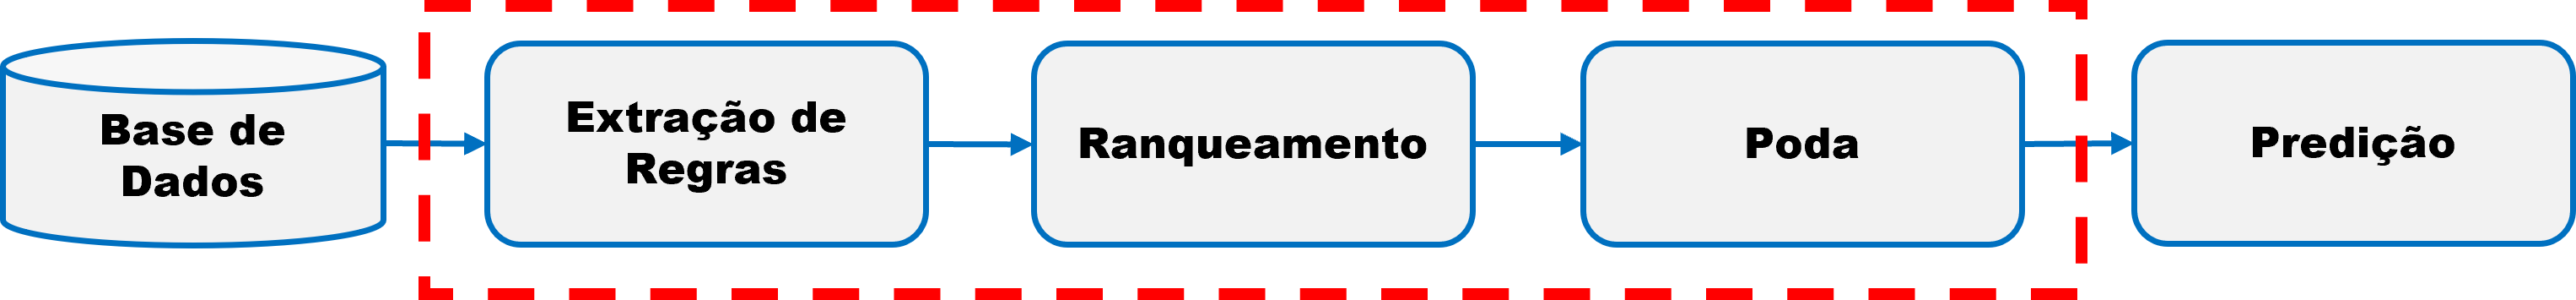
\includegraphics[width=\linewidth]{figuras/fluxo-geral.png}
    \caption{Fluxo geral de indução e predição de um classificador associativo.}
    \label{fig:fluxo_cba}
\end{figure}

No contexto desta dissertação, a seleção de atributos é realizada antes da indução do classificador associativo. Dessa forma, a redução do conjunto de atributos pode alterar os itens disponíveis para a geração de RACs e, consequentemente, influenciar tanto o desempenho preditivo quanto a quantidade e a estrutura das regras produzidas. Esses efeitos motivam a avaliação conjunta do desempenho e da complexidade dos classificadores obtidos após a aplicação do EFS4AC.

%%%%%%%%%%%

%%%%%%%%%%%
\section{Seleção de Atributos}\label{sec:fs} 

A seleção de atributos (\textit{feature selection} (FS))\footnote{Este trabalho utilizará os termos em português e inglês indistintamente.} é uma técnica de pré-processamento amplamente utilizada em aprendizado de máquina (AM), particularmente em conjuntos de dados de alta dimensionalidade \cite{Dhal2022,10.1007/978-3-031-23092-9_12,BARBIERI2024123667}. Seu objetivo consiste em identificar um subconjunto de atributos relevantes a partir do conjunto original, buscando, quando possível, reduzir a redundância entre eles, preservar ou melhorar o desempenho preditivo e reduzir a complexidade dos modelos \cite{Theng2024,Emmoh2024}.

No contexto da classificação associativa, conforme discutido na Seção~\ref{sec:ca}, a redução do número de atributos pode contribuir para diminuir o espaço de busca de regras e a complexidade dos classificadores induzidos. Dessa forma, a aplicação de métodos de FS pode proporcionar diferentes benefícios, entre os quais se destacam:
%%%%%%%%%%%%%%%%%%%%%%%%
\begin{itemize}
    \item \textbf{redução da complexidade e do custo computacional}: a diminuição do número de atributos pode reduzir o espaço de busca e o tempo de treinamento dos algoritmos \cite{Theng2024};

    \item \textbf{melhoria do desempenho e redução do risco de \textit{overfitting}}: a remoção de atributos ruidosos ou irrelevantes pode favorecer a capacidade de generalização dos modelos \cite{Dhal2022};

    \item \textbf{aumento da interpretabilidade e apoio à descoberta de conhecimento}: a utilização de um subconjunto menor de atributos pode facilitar a compreensão dos modelos e a identificação de características relevantes para o problema \cite{Dhal2022,KHAIRE20221060}.
\end{itemize}
%%%%%%%%%%%%%%%%%%%%%%%%

Três são as principais abordagens existentes para realização de FS, a saber \cite{Tan2020,Theng2024}: \textbf{filtro}, \textbf{\textit{embedded}} e \textbf{\textit{wrapper}}. A escolha da abordagem de FS é um ponto crítico, pois ela influencia diretamente a estabilidade do subconjunto de atributos selecionados e o desempenho final do modelo \cite{KHAIRE20221060,BARBIERI2024123667}. Em geral tem-se que:
\begin{itemize}
    \item \textbf{filtro}: constitui a abordagem mais simples e computacionalmente eficiente para a seleção de atributos. Os métodos existentes são independentes do algoritmo de AM que será utilizado \cite{Dhal2022,10.1007/978-3-031-23092-9_12,Theng2024,EBRAHIMIWARKIANI2025129372};
    
    \item \textbf{\textit{wrapper}}: utiliza um algoritmo de AM como mecanismo de avaliação de diferentes subconjuntos de atributos, sendo, portanto, dependente de um algoritmo base. Essa abordagem envolve a indução de múltiplos modelos, o que a torna mais custosa computacionalmente \cite{Theng2024};
    
    \item \textbf{\textit{embedded}}: realiza a seleção de atributos durante o processo de indução do modelo, sendo também dependente do algoritmo utilizado \cite{bashir2022novel,Theng2024}. Nessa abordagem, a relevância dos atributos é incorporada ao mecanismo de treinamento do modelo, como ocorre em árvores de decisão, métodos baseados em regularização e \textit{ensembles} de árvores. Em geral, métodos \textit{embedded} apresentam menor custo computacional que abordagens \textit{wrapper}, pois a seleção é integrada ao treinamento do modelo, embora os subconjuntos obtidos tendam a ser mais dependentes do algoritmo empregado.
\end{itemize}

Neste trabalho, são utilizados métodos de filtro como componentes do EFS4AC, devido à sua independência em relação ao algoritmo de classificação e à sua eficiência computacional. Esses métodos avaliam a relevância dos atributos por meio de critérios estatísticos, informacionais ou de dependência, sem utilizar diretamente o desempenho do classificador como função de avaliação \cite{SolorioFernandez2020,Bouchlaghem2022,Theng2024}.

Em abordagens baseadas em \textit{ranking}, os atributos recebem pontuações ou posições de acordo com o critério adotado. A partir dessa ordenação, um subconjunto pode ser definido mediante um limiar (\textit{threshold}) ou pela seleção de um número predefinido de atributos \cite{geng2007feature,jovic2015review,Theng2024}. Entretanto, a definição do subconjunto final constitui uma decisão adicional, uma vez que o \textit{ranking}, isoladamente, não determina quantos atributos devem ser selecionados.

Os métodos de filtro podem ser classificados em \textbf{univariados} e \textbf{multivariados} \cite{SolorioFernandez2020,Theng2024}. Os métodos univariados avaliam cada atributo individualmente, sem considerar explicitamente suas relações com os demais atributos. Já os métodos multivariados consideram relações entre atributos durante o processo de seleção, podendo incorporar critérios de redundância, dependência e interação \cite{SolorioFernandez2020,Dhal2022,Theng2024}.

Entre as principais vantagens dos métodos de filtro destacam-se a eficiência computacional e a independência em relação ao algoritmo de classificação, características que favorecem sua utilização em diferentes conjuntos de dados e modelos preditivos \cite{Dhal2022,Theng2024}. Por outro lado, os métodos univariados apresentam limitações na identificação de redundâncias e interações entre atributos, enquanto os métodos multivariados podem apresentar maior custo computacional. Além disso, diferentes critérios de avaliação podem produzir ordenações distintas dos atributos, e a escolha do ponto de corte pode influenciar a qualidade do subconjunto selecionado \cite{KHAIRE20221060,Theng2024}. Essa diversidade de critérios e resultados constitui uma das motivações para a combinação de diferentes métodos de seleção de atributos, conforme discutido na próxima subseção.

%%%%%%%%%%%%%%%%%%%%%
\subsection{\textit{Ensemble Feature Selection}}
\label{subsec:efs}

O \textit{Ensemble Feature Selection} (EFS) estende o princípio de aprendizado por \textit{ensemble} ao problema de seleção de atributos, combinando os resultados produzidos por múltiplos seletores-base para obter uma avaliação conjunta da relevância dos atributos \cite{bolon2019ensembles,salman2026review}. A motivação para o uso de EFS decorre do fato de que diferentes métodos de FS podem avaliar os atributos segundo critérios distintos e, consequentemente, produzir diferentes \textit{rankings} ou subconjuntos de atributos. Assim, em vez de depender exclusivamente do resultado de um único seletor, um \textit{ensemble} combina múltiplas avaliações com o objetivo de obter uma solução consensual e reduzir a variabilidade do processo de seleção, favorecendo maior robustez e estabilidade \cite{bolon2019ensembles,salman2026review}.

Diferentemente das abordagens filtro, \textit{wrapper} e \textit{embedded}, que caracterizam a forma como os atributos são avaliados e selecionados, o EFS constitui uma estratégia de combinação de múltiplos métodos de FS. Dessa forma, um EFS pode ser composto por seletores pertencentes a uma mesma abordagem ou a diferentes abordagens, combinando, por exemplo, métodos filtro, \textit{wrapper} e \textit{embedded}.

A diversidade entre os componentes de um EFS pode ser introduzida, principalmente, por meio de duas estratégias \cite{bolon2019ensembles}. Nos \textit{ensembles} homogêneos, um mesmo método de FS é aplicado sob diferentes condições, como diferentes amostras do conjunto de treinamento ou configurações do método, produzindo resultados que são posteriormente combinados. Nos \textit{ensembles} heterogêneos, por sua vez, diferentes métodos de FS são aplicados sobre o mesmo conjunto de dados, permitindo que critérios distintos de avaliação dos atributos contribuam para o resultado final. A Figura~\ref{fig:efs_homogeneo_heterogeneo} ilustra essas duas estratégias. Na Figura~\ref{fig:efs_homogeneo_heterogeneo}, $R_1,\ldots,R_k$ representam os \textit{rankings} produzidos pelo mesmo seletor sob diferentes condições no EFS homogêneo, enquanto $R_1,\ldots,R_m$ representam os \textit{rankings} obtidos por diferentes seletores no EFS heterogêneo. Em ambos os casos, os resultados individuais são encaminhados a uma estratégia de agregação, responsável por produzir uma representação consensual da importância dos atributos.

%%%%%%%%%%%%%%
\begin{figure}[htb]
    \centering
    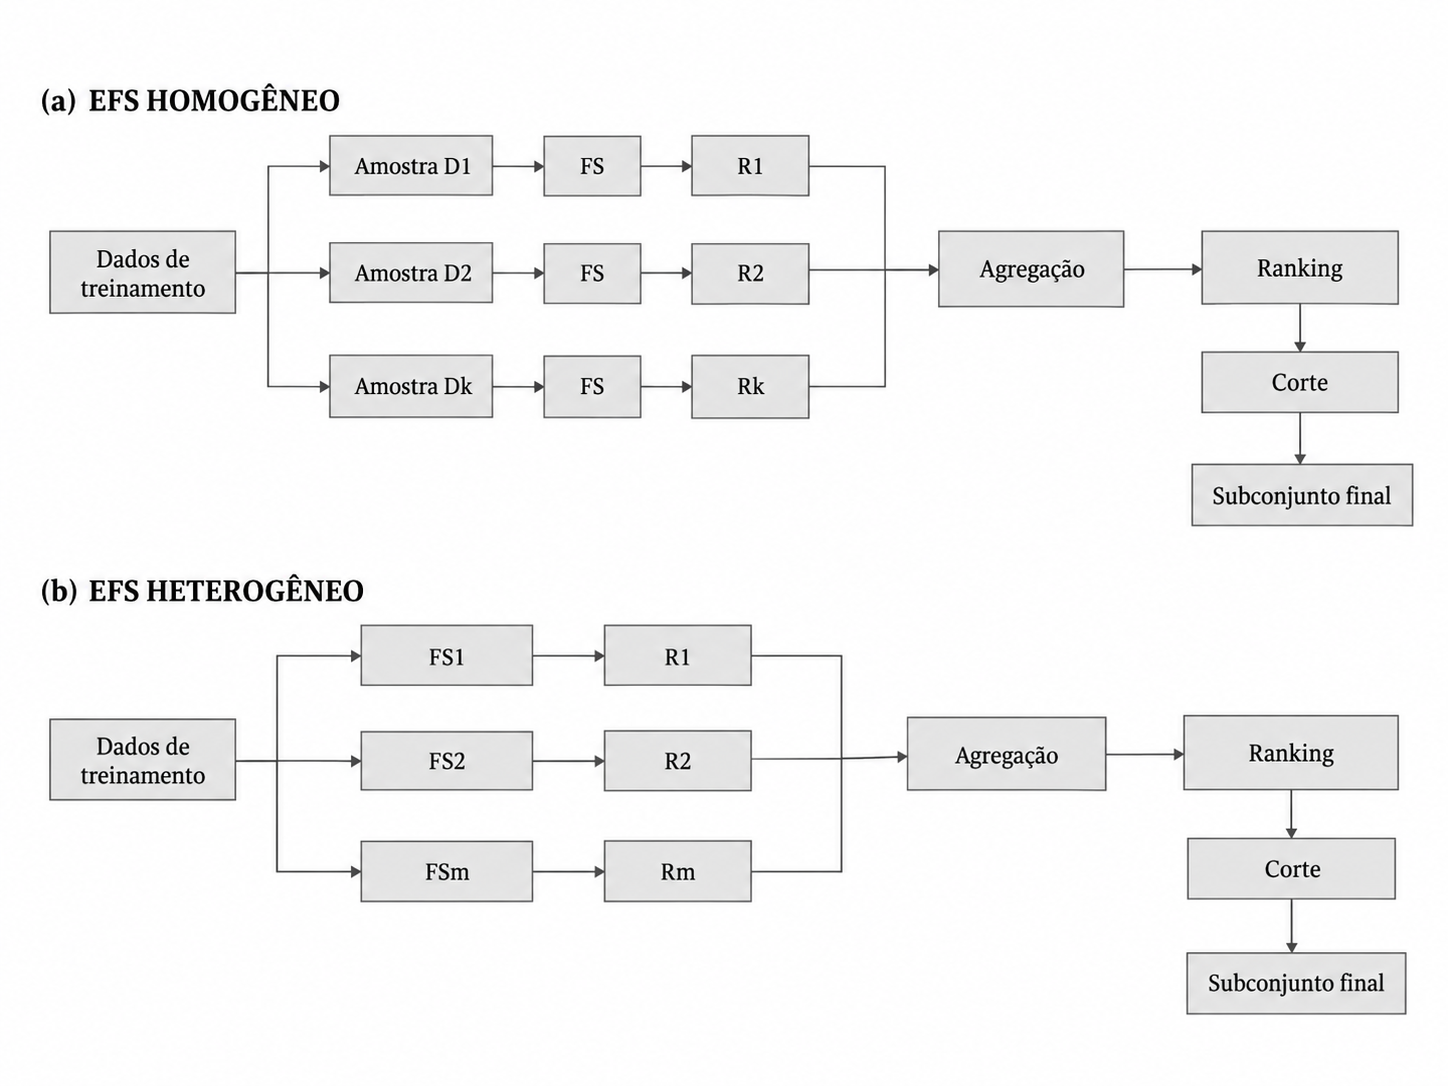
\includegraphics[width=\textwidth]
    {figuras/efs_homogeneo_heterogeneo.png}
    \caption{Estruturas gerais de \textit{Ensemble Feature Selection} homogêneo e heterogêneo. Elaborado pelo autor com base em \citeonline{bolon2019ensembles}.}
    \label{fig:efs_homogeneo_heterogeneo}
\end{figure}
%%%%%%%%%%%%%%

A forma de agregação depende do tipo de saída fornecida pelos seletores-base. Quando os métodos produzem subconjuntos de atributos, esses resultados podem ser combinados diretamente por estratégias de consenso. Quando produzem rankings ou pontuações (scores), diferentes métodos de agregação podem ser utilizados para gerar uma avaliação global da importância dos atributos \cite{bolon2019ensembles}. Nesse segundo caso, torna-se necessária uma etapa adicional de definição do subconjunto final (\textit{thresholding}), responsável por converter a avaliação agregada em um conjunto de atributos selecionados.

Assim, a construção de um EFS envolve diferentes decisões metodológicas, incluindo a composição do conjunto de seletores, a geração de diversidade entre seus componentes, a estratégia de agregação dos resultados individuais e o critério empregado para determinar o subconjunto final de atributos. Essas decisões podem influenciar propriedades importantes do processo de seleção, como estabilidade, robustez e dimensionalidade do subconjunto obtido, bem como o desempenho dos modelos induzidos.

%%%%%%%%%%%

%%%%%%%%%%%
%%%%%%%%%%%%%%%%%%%%%%%%%%%
\section{Critérios de Avaliação}
\label{met_avaliacao}
%%%%%%%%%%%%%%%%%%%%%%%%%%%
%%%teria mais o custo computacional

A avaliação de uma estratégia de seleção de atributos aplicada à classificação não deve considerar apenas o desempenho preditivo do modelo resultante. No contexto deste trabalho, a análise envolve diferentes dimensões, incluindo a capacidade classificatória, a redução da dimensionalidade, a estabilidade do processo de seleção e a complexidade do classificador associativo obtido. Esses critérios permitem avaliar não apenas se a seleção preserva ou melhora a capacidade de predição, mas também seus efeitos sobre o subconjunto de atributos e a estrutura do modelo baseado em regras.

O desempenho preditivo deve ser avaliado sobre dados não utilizados durante o treinamento, permitindo estimar a capacidade de generalização do classificador. Entre as medidas comumente utilizadas estão precisão, revocação e medida-F, que, em problemas multiclasse, podem ser agregadas por estratégias como micro, macro e macro ponderada. Neste trabalho, destaca-se a medida F1-macro, que atribui o mesmo peso a cada classe no cálculo da média dos valores de F1. Para obter estimativas mais confiáveis, podem ser empregados protocolos como \textit{holdout} e validação cruzada (\textit{cross-validation}), incluindo sua versão estratificada. Uma discussão detalhada dessas medidas e estratégias pode ser encontrada em \citeonline{Tan2020}.

No contexto de seleção de atributos, outra dimensão relevante corresponde à redução da dimensionalidade. Seja $F$ o conjunto original de atributos e $S \subseteq F$ o subconjunto selecionado, o percentual de redução pode ser expresso conforme a Equação~\ref{eq:red-fs}. Essa medida permite verificar o quanto uma estratégia de FS reduz o espaço original de atributos. No caso da classificação associativa, essa redução pode produzir efeitos adicionais, uma vez que os atributos selecionados determinam os itens disponíveis para a mineração e, consequentemente, podem modificar o número de \textit{itemsets} e as regras produzidas.

%%%%%%%
\begin{equation}\label{eq:red-fs}
    \text{Redu\c{c}\~{a}o(\%)} =
    \left(
    1 - \frac{|S|}{|F|}
    \right) \times 100
\end{equation}
%%%%%%%

Outro aspecto relevante para métodos de FS e EFS é a estabilidade da seleção. A estabilidade refere-se à capacidade de um método produzir subconjuntos semelhantes quando pequenas alterações são realizadas nos dados de treinamento. Uma estratégia de seleção pode apresentar desempenho preditivo semelhante entre diferentes execuções e, ainda assim, selecionar atributos substancialmente distintos. Em EFS, essa propriedade é particularmente relevante, uma vez que a combinação de múltiplos seletores pode contribuir para reduzir a variabilidade associada às decisões individuais de seleção. A estabilidade pode ser avaliada por meio de medidas que quantificam a similaridade entre os subconjuntos de atributos obtidos em diferentes execuções do processo de seleção.

Em algoritmos baseados em regras, a avaliação pode considerar também propriedades relacionadas à complexidade e à interpretabilidade do modelo. Embora modelos baseados em regras sejam frequentemente considerados inerentemente interpretáveis, a utilização de regras não garante, por si só, uma representação simples \cite{Rudin2019,margot2021interpretability,molnar2022}. Um classificador pode conter um grande número de regras ou regras extensas, tornando sua inspeção difícil. Por esse motivo, propriedades estruturais do modelo são frequentemente utilizadas como aproximações da complexidade interpretativa.

No contexto da classificação associativa, a quantidade de regras é uma dessas medidas e tem sido empregada em diferentes trabalhos \cite{Agnol:2024,math11183978,momac,app12189055,Building2020,DBLP:journals/access/Rajab19,DBLP:conf/kdd/LakkarajuBL16}. Entretanto, o número de regras não deve ser interpretado isoladamente como uma medida completa de interpretabilidade, pois outras propriedades, como o comprimento dos antecedentes e a redundância entre regras, também podem influenciar a complexidade do modelo.

Dessa forma, a avaliação das estratégias investigadas neste trabalho considera diferentes perspectivas complementares. O desempenho preditivo indica a capacidade de generalização do classificador; a redução dimensional caracteriza a capacidade do método de FS em restringir o espaço de atributos; a estabilidade avalia a consistência da seleção diante de perturbações nos dados; e as propriedades estruturais do classificador associativo permitem analisar os efeitos da seleção sobre a complexidade do modelo baseado em regras.

%%%%%%%%%%%